\documentclass[12pt,a4paper]{article}
\usepackage[italian]{babel}
\usepackage[T1]{fontenc}
\usepackage[latin1]{inputenc}
\usepackage{graphicx}
\usepackage{amsmath}
\usepackage{subfig}
\usepackage[a4paper,top=1.5cm,bottom=1.4cm,left=1.4cm,right=1.4cm]{geometry}
\date{}
\begin{document}
\title{Ipersonica\\ Esercitazione 5 \\ Prof.re Renato Paciorri}
\author{Matteo Hakimi 1455230}
\maketitle
\begin{figure}[htbp]
\centering

\includegraphics[width=100mm]{Immagini/1}
\end{figure}
\newpage
\tableofcontents
\newpage
\section{Introduzione}
Si vuole studiare il flusso all'interno dello strato limite in prossimit� del punto di ristagno, formatosi su un corpo tozzo con raggio di curvatura in prossimit� del punto di ristagno pari a $r=1$ m, di una miscela reagente in campo ipersonico. 
\section{Flusso reagente nello strato limite}
In questa sezione ci dedicheremo allo studio di una miscela composta da azoto molecolare $N_{2}$ e atomico $N$.\\
In particolare si supporr� che le temperature all'interno dello strato d'urto siano tali ($T_{e}=10000K$) da indurre la dissociazione completa dell'azoto $\alpha=1$.\\
Le ipotesi semplificative che verranno adottate sono:\\
$\bullet$\quad Nella zona esterna lo strato limite, il flusso � in condizioni di equilibrio chimico.\\
$\bullet$\quad I fenomeni vibrazionali non verranno considerati.\\
$\bullet$\quad La temperatura di parete del corpo � relativamente bassa ($T_{w}=1000K$), tale da indurre la ricombinazione completa dell'azoto (parete completamente catalica $\alpha_{w}=0$).\\
Introducendo le seguenti adimensionalizzazioni:\\
$$f'(\eta)=\frac{u}{u_{e}},\quad g(\eta)=\frac{h}{h_{e}},\quad \theta(\eta)=\frac{T}{T_{e}},\quad$$\\
con:\\
$$\eta=\frac{u_{e}}{\sqrt{2\xi}}\iiint_0^y \rho(y)\,dy$$
$$\xi=\int_{0}^{x}\rho_{e}u_{e}\mu_{e},dx$$
$${\partial{f}\over{\partial \eta}}=f^{'}$$
Possiamo riscivere il sistema di equazioni di Navier Stokes, e la generica equazione della specie $i^{-esima}$ attraverso le variabili appena introdotte, che di fatto semplificano il problema considerato; infatti questo metodo ci permette di riscrivere il sistema di equazioni alle derivate parziali in un sistema alle derivate ordinarie.\\
In particolare si ha:\\
$$(lf'')'+ff''+\frac{1}{2}\left[\frac{\rho_{e}}{\rho}-(f')^2\right]=0$$
$$(\frac{l}{P_{r}}g')'+fg'+\left[\frac{l}{P_{r}}\sum_{i}\frac{c_{ei}}{h_{e}}\left(h_{i}-\Delta h_{i}^0\right)\left(L_{e}-1\right)c_{i}'\right]=0$$
$$(\frac{l}{P_{r}}L_{e}\alpha)+f\alpha'-\frac{\dot{W_{\alpha}}}{2\frac{du_{e}}{dx}\rho}=0$$\\\\
dove con $P_{r}$ si � indicato il numero di Prandtl, $L_{e}=\frac{\rho D_{12}C_{p}}{\mu}$ il numero di Lewis e l � definito come:\\
$$l:=\frac{\rho\mu}{\rho_{w}\mu_{w}}$$
Mentre il termine $\dot{w}_{\alpha}$, rappresenta il termine reagente, che ne caso della dissociazione/ricombinazione dell'azoto � definito come:\\
$$\dot{w}_{\alpha}=\rho(1+\alpha)^2\left[k_{f}(T)\frac{(1-\alpha)p}{(1+\alpha)R_{0}T}-4k_{b}(T)\left(\frac{\alpha p}{(1+\alpha)R_{0}T}\right)^2\right]$$
Inoltre supponendo che la viscosit� e la pressione non varino, � possibile esprimere $l$ in funzione di $\alpha$ e $\theta$, infatti si ha:\\
$$l=\frac{1+\alpha_{w}}{1+\alpha}\frac{T_{w}}{T_{e}}\frac{1}{\theta}$$
Mentre:\\
$$g=\frac{h}{h_{e}}=\frac{C_{p}T+\alpha\Delta h_{N}^0}{C_{pe}T_{e}+\alpha_{e}\Delta h_{N}^0}$$
Da cui si ricava:\\
$$\theta=\frac{h_{e}g-\alpha\Delta h_{N}^0}{C_{p}T_{e}}$$
con:\\
$$C_{p}=\frac{7+3\alpha}{4}\frac{R_{0}}{PM_{N}}$$\\
Inoltre:\\
$$\frac{\rho_{e}}{\rho}=\frac{1+\alpha}{1+\alpha_{e}}\theta$$    
Assumendo un numero di Lewis e Prandtl pari ad 1, e sapendo che possiamo scrivere: $$\frac{du_{e}}{dx}=\frac{1}{r}\sqrt{\frac{2(p_{e}-p_{\infty})}{\rho_{e}}}$$
Il sistema di equazioni subisce una notevole semplificazione, inoltre al fine di ricondurre il sistema in un sistema di 7 equazioni differenziali al primo ordine, introduciamo le seguanti variabili:\\
$$F=f',\quad A=lF',\quad B=lg',\quad C=l\alpha'$$
Il sistema di equazioni differenziali in forma normale diventa:\\
$$f'=F$$
$$F'=\frac{A}{l}$$
$$g'=\frac{B}{l}$$
$$\alpha'=\frac{C}{l}$$
$$A'=-f\frac{A}{l}+\frac{1}{2}F^2+b_{1}$$
$$B'=-f\frac{B}{l}$$
$$C'=-f\frac{C}{l}+b_{3}$$
con le seguenti condizioni al contorno:\\
$\bullet$\quad $\eta=0$
$$f(0)=0$$
$$F(0)=0$$
$$g(0)=g_{w}$$
$$\alpha(0)=0$$
$\bullet$\quad $\eta=\infty$
$$F(\infty)=1$$
$$g(\infty)=1$$
$$\alpha(\infty)=1$$
In genere in questo tipo di problemi condizioni al contorno asintotiche, quello che si usa � la tecnica di over-shooting, che consiste di ricondurre le condizioni asintotiche a delle condizione iniziale, assegnando come primi valori dei valori tentativo di $A(0)=A_{i}$, $B(0)=B_{i}$ e $C(0)=C_{i}$ iterando fino a convergenza della $F$, $g$ e $\alpha$ all'infinito.\\
Si implementa su codice Matlab il sistema di equazioni e relative condizioni al contorno.\\
Scegliendo inizialmente come valori tentativo:\\
$$A(0)=0.5,\quad B(0)=0.5,\quad C(0)=0.5 $$
E procedendo, variando dal principio $C(0)$ in modo da avere $\alpha(\infty)=1$, e successimanvente $B(0)$ e $A(0)$, facendo attenzione ai valori assunti dai valori asintotici, si ottiene:\\
$$A(0)=0.23017,\quad B(0)=0.1780,\quad C(0)=0.1812 $$
rispettivamente con:
$$F(\infty)=1,\quad g(\infty)=1,\quad \alpha(\infty)=1$$ 
Vengono riportati in figura gli andamenti di $F=F(\eta)$, $g=g(\eta)$ e $\alpha=\alpha(\eta)$ rispettivamente.\\
\begin{figure}[htbp]
	\centering
	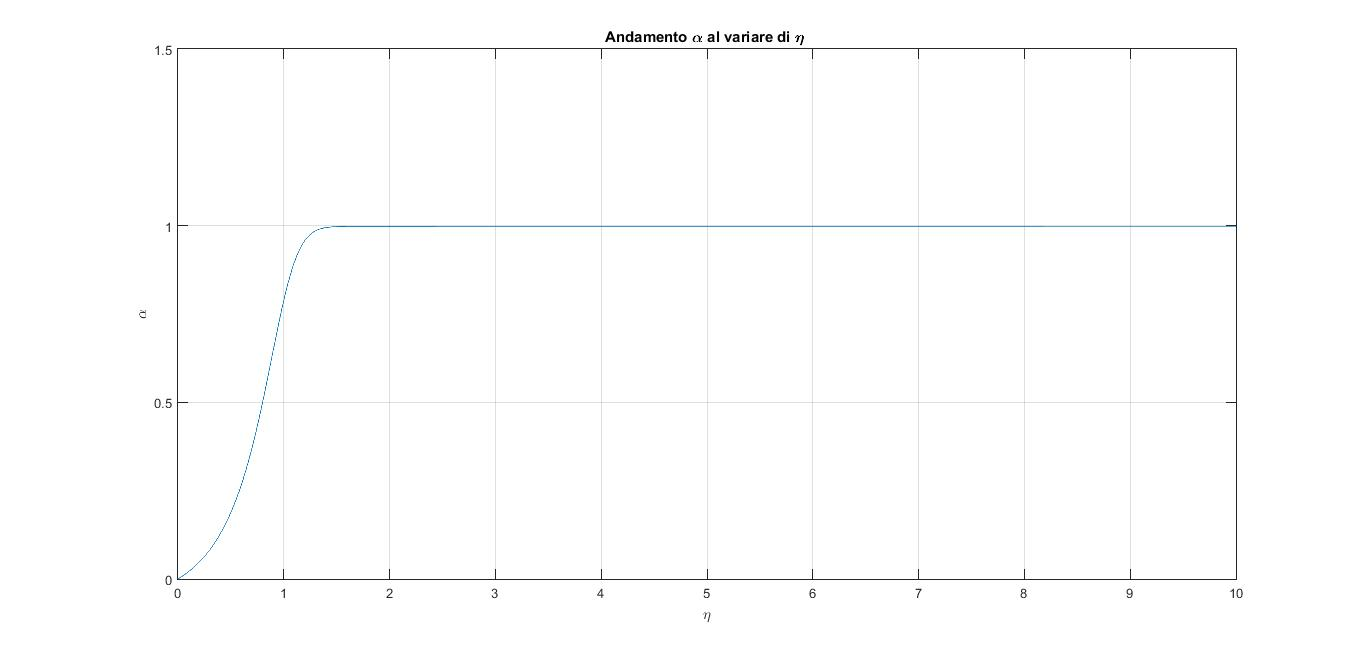
\includegraphics[width=150mm]{Immagini/alpha}
	\caption{Andamento del grado di dissociazione in funzione di $\eta$}
\end{figure}
\begin{figure}[htbp]
	\centering
	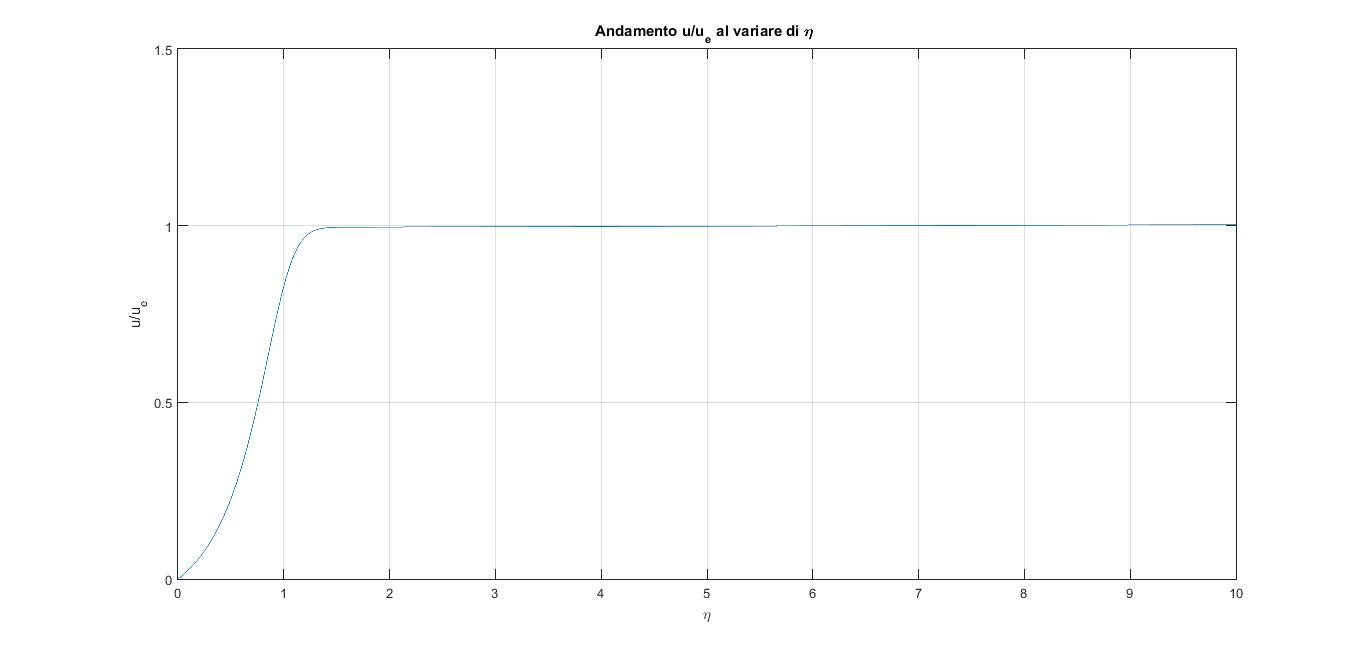
\includegraphics[width=150mm]{Immagini/F}
	\caption{Andamento di $u/u_{e}$ in funzione di $\eta$}
\end{figure}
\begin{figure}[htbp]
	\centering
	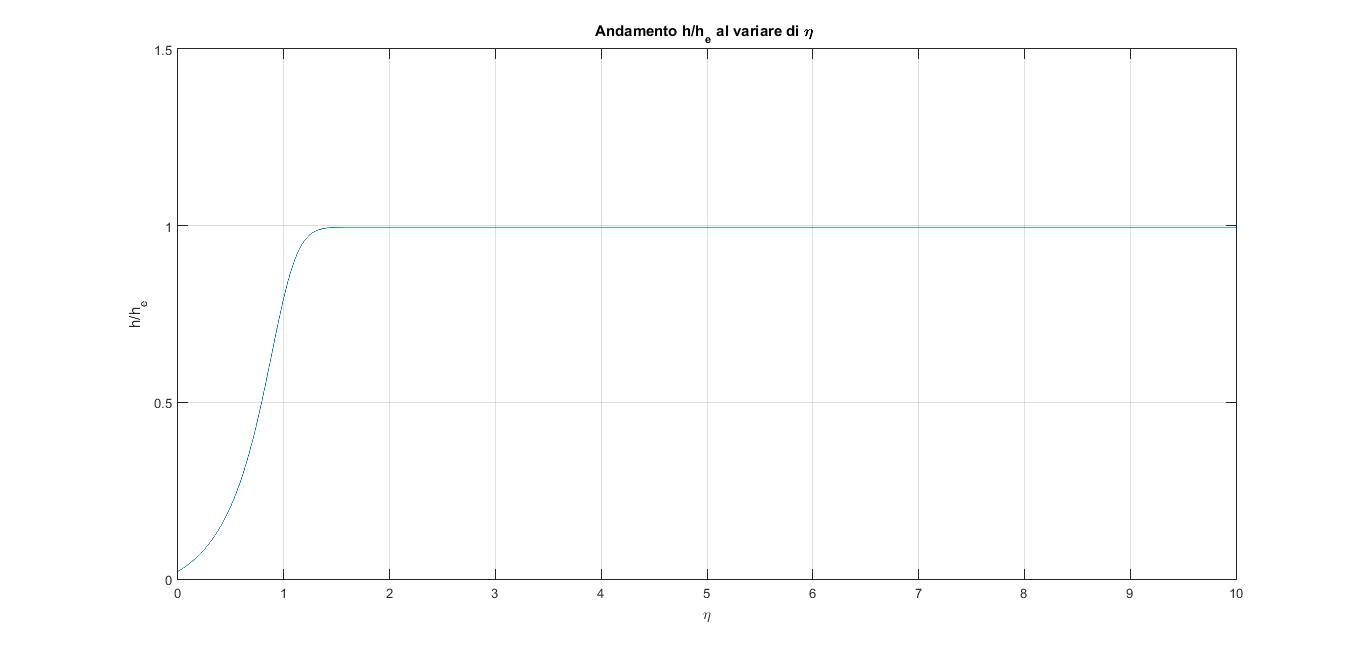
\includegraphics[width=150mm]{Immagini/g}
		\caption{Andamento di $h/h_{e}$ in funzione di $\eta$}
\end{figure}
\end{document}